\chapter{认识 Bumi}
\setchapterheader{第\thechapter 章\quad 认识 Bumi}

\begin{intro}
认识机器人的自由度、版本、接口和机载计算机，查阅相机、电池与充电器参数。
\end{intro}
\section{部件与自由度}
Bumi 全身共有 21 个自由度。这里的自由度可以理解为一个独立控制的关节转动方向。单臂有 4 个，单腿有 6 个，腰部有 1 个，因此总数为 $2\times4+2\times6+1=21$。
\begin{itemize}
\item 手臂：肩关节 pitch、肩关节 roll、上臂 yaw、肘关节 pitch。
\item 腿部：髋关节 pitch、髋关节 roll、大腿 yaw、膝关节 pitch、踝关节 pitch、踝关节 roll。
\item 腰部：腰关节 yaw。
\end{itemize}
pitch、roll 和 yaw 分别表示俯仰、横滚和偏航。具体关节的正方向要结合模型坐标系阅读，电机编号、名称和范围见附录\ref{app:joints}。
\begin{figure}[H]
\centering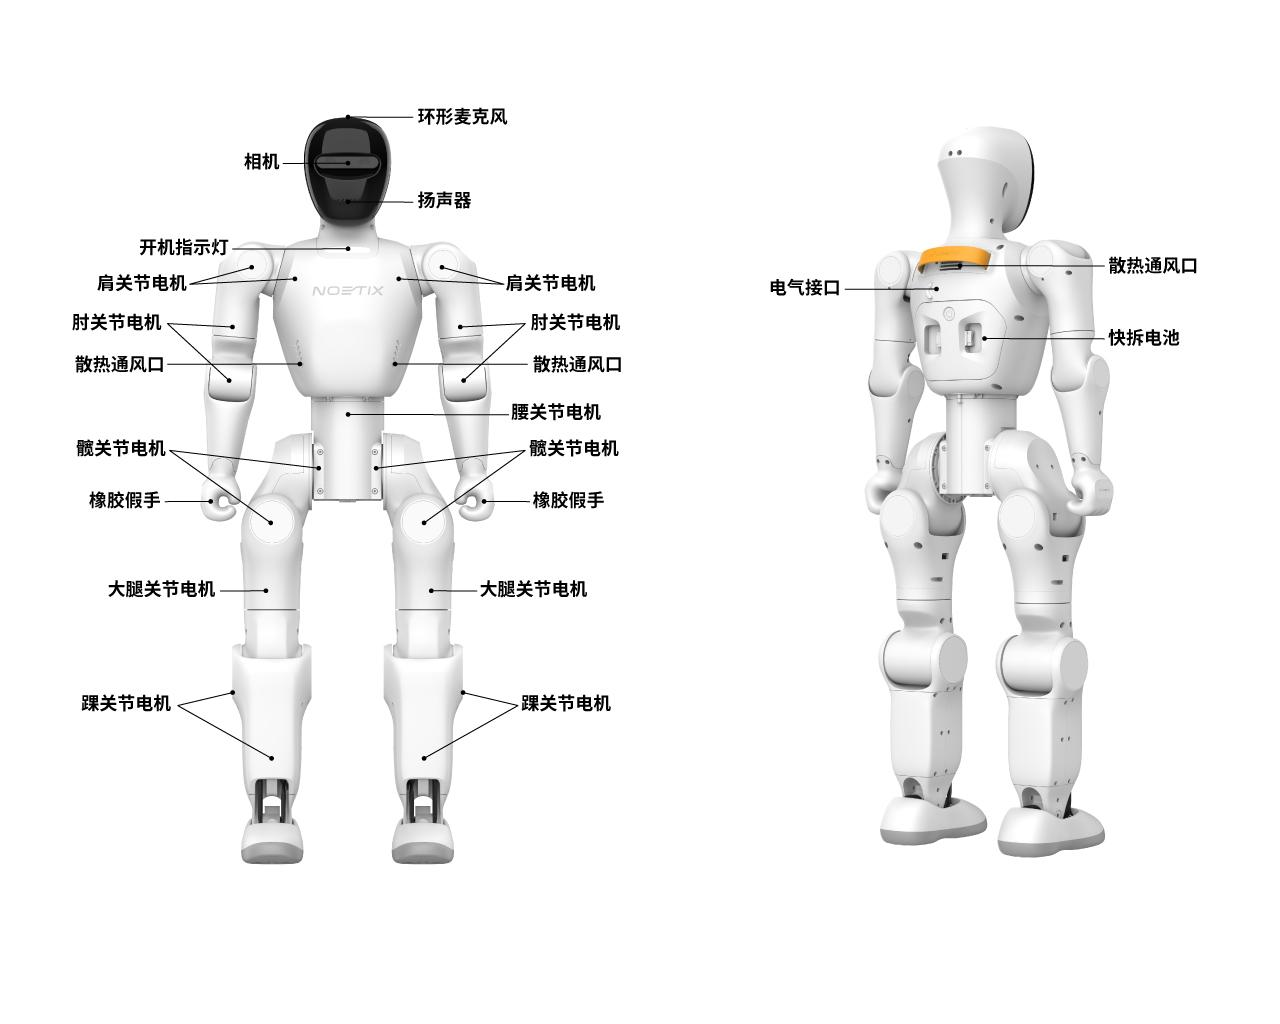
\includegraphics[width=0.72\linewidth]{images/bumi-components.jpg}
\caption{Bumi 部件示意图}
\end{figure}
\section{整机参数与版本}

\begingroup\small\renewcommand{\arraystretch}{1.15}
\begin{longtable}{@{}P{0.32\linewidth}P{0.61\linewidth}@{}}
\toprule
\textbf{项目} & \textbf{参数} \\
\midrule\endhead
站立尺寸（高、宽、厚） & 约 98 cm $\times$ 35 cm $\times$ 20 cm \\
带电池重量 & 约 17 kg \\
总自由度 & 21；单臂 4、单腿 6、腰部 1 \\
关节通信 & EtherCAT 与 CAN FD \\
整机规格表中的最大关节扭矩 & 70 N·m \\
大腿与小腿长度 & 合计约 513 mm \\
手臂长度 & 约 312 mm \\
供电 & 快拆锂电池；标称续航 2--3 小时 \\
感知与交互 & IMU、相机、麦克风阵列、扬声器、APP 与 OTA \\
\bottomrule\end{longtable}\endgroup

官方外形尺寸图标注的整机高度为 988 mm，宽度为 350.46 mm，侧向厚度为 203.20 mm。整机概览采用取整尺寸；安装与结构设计可在\officiallink{J7iRd3pqzo6ICqxdHyHcfakQnff}{外观件尺寸图}中查看完整尺寸标注。关节控制使用附录中的逐关节参数。

\begingroup\small\renewcommand{\arraystretch}{1.15}
\begin{longtable}{@{}P{0.22\linewidth}P{0.27\linewidth}P{0.42\linewidth}@{}}
\toprule
\textbf{项目} & \textbf{标准版} & \textbf{教育版} \\
\midrule\endhead
基础算力 & 6 TOPS & 6 TOPS，部分型号另配 67 / 117 TOPS 算力板 \\
算力模块 & 无独立 Jetson 算力板 & Jetson Orin Nano Super / NX；部分型号无算力板 \\
相机 & \code{DC_V93} & RealSense D435i；EDU\_Air 除外 \\
图传 & 通过 APP 使用 & 开发时可在算力板访问相机硬件 \\
HighController & 支持 & 支持 \\
LowController & 未开放 & 支持 \\
\bottomrule\end{longtable}\endgroup

\section{背部电气接口}
背部提供 1 个 RJ45 千兆以太网口、2 个 USB 3.0 接口和 1 个 HDMI 接口。RJ45 采用 1000BASE-T。配有算力板的版本，背部接口连接算力板；未配算力板的版本，接口连接运控板。接线位置见\officiallink{doxcnqSG6s08595TTZSMDbgjqRb}{官方电气接口图}。
\section{机载计算机}
机器人内部的运控板负责运动控制。教育版中的 Jetson 算力板用于运行用户程序，两者通过网络通信。

\begingroup\small\renewcommand{\arraystretch}{1.15}
\begin{longtable}{@{}P{0.17\linewidth}P{0.23\linewidth}P{0.25\linewidth}P{0.25\linewidth}@{}}
\toprule
\textbf{项目} & \textbf{运控板} & \textbf{算力板 Nano Super} & \textbf{算力板 NX} \\
\midrule\endhead
平台 & RK3576 & Jetson Orin Nano Super & Jetson Orin NX \\
默认 IP & \code{192.168.55.102} & \code{192.168.55.101} & \code{192.168.55.101} \\
算力 & 6 TOPS & 67 TOPS & 117 TOPS \\
主频 & 2.4 GHz & 1.7 GHz & 2.0 GHz \\
内存与存储 & 8 + 64 GB & 8 + 128 GB & 16 + 128 GB \\
用户登录 & 通过 SDK 接口访问功能 & 用户 \code{noetix} & 用户 \code{noetix} \\
\bottomrule\end{longtable}\endgroup

算力板出厂账户为 \code{noetix}，初始密码为 \code{bumi}。开发时登录算力板，运动命令通过 SDK 发给运控板。
\section{相机}
标准版使用 DC\_V93 USB 摄像模组，最高有效像素为 $2592\times1944$。教育版的 D435i 使用方法见第\ref{chap:camera}章。

\begingroup\small\renewcommand{\arraystretch}{1.15}
\begin{longtable}{@{}P{0.29\linewidth}P{0.63\linewidth}@{}}
\toprule
\textbf{DC\_V93 项目} & \textbf{参数} \\
\midrule\endhead
感光尺寸与像素尺寸 & 1/4 英寸；$1.4\,\mu$m $\times$ $1.4\,\mu$m \\
图像格式 & MJPEG；YUV2（YUYV） \\
接口 & USB 2.0 High Speed \\
对焦 & 固定 / AF \\
中心清晰度 & 800 LW/PH（Center） \\
信噪比与动态范围 & 36 dB；71.6 dB \\
灵敏度与最低照度 & 1.4 V/lux-sec @ 550 nm；0.5 lux \\
自动控制 & 支持自动曝光、自动白平衡、自动增益 \\
镜头 & 焦距 6.78 mm；光圈 F2.4；对角视场角 32.6° \\
可调参数 & 亮度、对比度、饱和度、色调、清晰度、伽马、白平衡、逆光对比、曝光度 \\
\bottomrule\end{longtable}\endgroup

\begingroup\small\renewcommand{\arraystretch}{1.15}
\begin{longtable}{@{}P{0.35\linewidth}P{0.26\linewidth}P{0.28\linewidth}@{}}
\toprule
\textbf{分辨率} & \textbf{MJPEG 帧率} & \textbf{YUV 帧率} \\
\midrule\endhead
$2592\times1944$ & 30 fps & 2 fps \\
$1920\times1080$ & 30 fps & 5 fps \\
$1280\times720$ & 30 fps & 8 fps \\
$848\times480$ & 30 fps & 20 fps \\
$640\times480$ & 30 fps & 30 fps \\
\bottomrule\end{longtable}\endgroup

\section{电池与充电器}

\begingroup\small\renewcommand{\arraystretch}{1.15}
\begin{longtable}{@{}P{0.3\linewidth}P{0.62\linewidth}@{}}
\toprule
\textbf{电池项目} & \textbf{参数} \\
\midrule\endhead
生产商 & 深圳格瑞普 \\
型号 & \code{GRP6752097-13S1P} \\
容量 & 5100 mAh \\
标称电压 & 48 V \\
重量 & 1360 g \\
\bottomrule\end{longtable}\endgroup

\begingroup\small\renewcommand{\arraystretch}{1.15}
\begin{longtable}{@{}P{0.3\linewidth}P{0.62\linewidth}@{}}
\toprule
\textbf{充电器项目} & \textbf{参数} \\
\midrule\endhead
型号 & TA300 Robot 智能充电器 \\
输入 & 100--240 V AC；50/60 Hz；4.5 A \\
支持电池 & LiPo / LiFe / LiHV；13S--16S \\
输出 & 35--72 V DC；7.5 A；最大 350 W \\
尺寸 & $172\times97\times46$ mm \\
重量 & $510\pm10$ g \\
工作模式 & 充电 \\
\bottomrule\end{longtable}\endgroup
